\documentclass[12pt]{article}
\usepackage{listings}
\usepackage[utf8]{inputenc}
\usepackage[T1]{fontenc}
\usepackage[polish]{babel}
\usepackage{url}
\usepackage{graphicx}

\title{Zastosowanie algorytmów ewolucyjnych do zagadnień
  kombinatorycznych na przykładzie problemu szeregowania zadań - sprawozdanie}
\author{Michał Karpiński, Maciej Pacut}
\date{Grudzień 2011}
\begin{document}
  \maketitle

\hyphenation{krzy-żo-wa-nia ma-szy-nie}

\section{Wstęp}
Problem szeregowania zadań ma kilka różnych wariantów. W niniejszej pracy zajmujemy się problemem typu {\em Flow Shop}.
Problem ten jest problemem planowania produkcji, w którym $n$ zadań musi zostać wykonanych na $m$ maszynach (jeden po drugim).
Danymi wejściowymi są $n$, $m$ oraz macierz $T$, gdzie $T[i][j]$ jest czasem wykonania zadania $i$ na maszynie $j$ $(i = 1..n, j = 1..m )$.
Czasy są nieujemne, stałe i nie zmianiają się podczas pracy maszyn. Problemem jest zminimalizowanie czasu 
pomiędzy rozpoczęciem wykonywania pierwszego zadania na pierwszej maszynie a zakończeniem wykonywania ostatniego zadania na ostatniej maszynie.
Dla naszego problemu przyjmujemy nastepujące założenia:

\begin{itemize}
  \item Każde zadanie musi być wykonane co najwyżej raz na maszynach $1, 2 ... m$ (w tej kolejności)
  \item Każda maszyna w danym momencie pracuje tylko nad jednym zadaniem
  \item Każde zadanie w danym momencie jest wykonywane na co najwyżej jednej maszynie
  \item Wykonywanie zadania nigdy nie jest zakłócone (przerwane)
  \item Czas pomiędzy przekazaniem zadania z jednej maszyny na drugą jest zerowy
\end{itemize}

Tak zdefiniowany problem jest NP-trudny. W niniejszej pracy prezentujemy algorytm ewolucyjny poszukujący przybliżonego rozwiązania.

\section{Schemat algorytmu ewolucyjnego}

Do rozwiązania problemu {\em Flow Shop} zastosowaliśmy algorytm
genetyczny SGA wykonujący się wg następującego schematu:

\begin{verbatim}
Losuj populację początkową
while(NOT Warunek Zakończenia)
{
  Krzyżowanie w obrębie populacji
  Mutacja osobników w populacji
  Zastąpienie populacji nową
}
\end{verbatim}

Rodzice dla opratorów krzyżowania są wybierani z prawdopodobieństwem
proporcjonalnym do wartości funkcji przystosowania kandydata.

Długość wymienianego łańcucha jest stałą i wynosi $\frac{1}{3}$ długości
permutacji. Losowane jest miejsce rozpoczęcia wymienianego łańcucha.

Mutacja jest przeprowadzana z prawdopodobieństwem 0.3.

\section{Operatory ewolucyjne}

Zostały wykorzystane operatory krzyżowania permutacji PMX, CX, OX.

\begin{itemize}
  \item {\em Partially-Matched Crossover (PMX)} - spójny blok genów z pierwszego rodzica jest mapowany na drugiego rodzica (w tym samym miejscu).
        Niektóre geny mogą się powtarzać, więc wykonuje się naprawienie permutacji poprzez serię transpozycji w obrębie chromosomów rodzicielskich.
  \item {\em Cycle Crossover (CX)} - ustalane są cykle między rodziecem pierwszym a drugim, następnie cykle są numerowane. Potomkowie są tworzeni poprzez
        kopiowanie genów należących do cykli nieparzystych (w sensie numeracji) i zamianie genów leżących na pozycjach należących do cykli 
        parzystych na geny drugiego rodzica (na tej samej pozycji)
  \item {\em Order Crossover Operator (OX)} - spójny blok genów z pierwszego rodzica jest mapowany na drugiego rodzica (w tym samym miejscu). Reszta genów jest
        przepisywana kolejno zaczynając od miejsca zakończenia mapowania, pomijając geny występujące w mapowaniu.
\end{itemize}

\noindent Operator mutacji aplikuje losową transpozycję do mutowanej permutacji.

\section{Funkcja celu}

Funkcją celu, czyli wartością, do której będzie dążył algorytm jest czas
pomiędzy rozpoczęciem wykonywania pierwszego zadania na pierwszej maszynie a
zakończeniem ostatniego zadania na ostatniej maszynie. To kryterium optymalizacyjne
nosi nazwę {\em makespan}. Będziemy posługiwali się następującymi oznaczeniami:

\begin{itemize}
  \item Dane rozwiązanie (permutacja $n$-elementowa): $\pi$
  \item Czas obróbki $i$-tego zadania na $j$-tej maszynie: $p_{\pi_i,j}$
  \item Czas zakonczenia $i$-tego zadania na $j$-tej masz: $C(\pi_i,j)$
  \item Kryterium optymalizacyjne: $C_{max}$: $C(\pi_n,m)$
\end{itemize}

Wartość funkcji $C_{max}$ wyraża się wzorem rekurencyjnym:

\begin{itemize}
  \item $C(\pi_1,1) = p_{\pi_1,1}$
  \item $C(\pi_i,1) = C(\pi_{i-1},1) + p_{\pi_i},1$
  \item $C(\pi_1,j) = C(\pi_1,j-1) + p_pi_1,j$
  \item $C(\pi_i,j) = max\{C(\pi_i,j-1),C(\pi_{i-1},j)\} + p_{\pi_i},j$
\end{itemize}

Warto zauważyć, że do obliczenia $C_{max}$ można zastosować algorytm dynamiczny. 

\section{Przeprowadzone testy}

\subsection{Dane testowe}

W celu ustalenia sprawności algorytmu SGA wykorzystane zostały zestawy testów prof. Erica Taillarda
(\url{http://mistic.heig-vd.ch/taillard/problemes.dir/ordonnancement.dir/ordonnancement.html}),
dla których znane są optymalne rozwiązania.

\begin{figure}
  \centering
    \begin{tabular}{ | c | c | c | }
      \hline                       
      Nazwa & N & M \\ \hline
      ta001-010 & 20 & 5 \\
      ta011-020 & 20 & 10 \\
      ta021-030 & 20 & 20 \\
      ta031-040 & 50 & 5 \\
      ta041-050 & 50 & 10 \\
      ta051-060 & 50 & 20 \\
      ta061-070 & 100 & 5 \\
      ta071-080 & 100 & 10 \\
      ta081-090 & 100 & 20 \\
      ta091-100 & 200 & 10 \\
      \hline
\end{tabular}
 \caption{Zestawy testowe, rozmiar danych}
  \label{tab:tests}
\end{figure}

W tabeli \ref{tab:tests} znajduje się uproszczony opis stu zestawów testowych użytych
podczas wykonywania eksperymentów ($N$ - ilość zadań, $M$ - ilość maszyn ). Przeprowadzono testy na różnych wielkościach populacji i dla różnych warunków stopu
(procentowa odległość od optimum).

\subsection{Znajdowanie optimum}

W celu ustalenia, czy nasza implementacja algorytmu SGA wykazuje cechy algorytmu ewolucyjnego wykonaliśmy serię niewielkich eksperymentów (dla małej liczby iteracji).
Wykres \ref{pic:plot1} przedstawia średnią wartość funkcji celu w populacji, w zależności od liczby iteracji. Widać wyraźnie, że populacja zbiega do pewnego ekstremum.
Liczne skoki wartości funkcji celu widoczne po osiągnięciu ekstremum, spowodowane są zastosowaniem operatora mutacji. Dzięki temu istnieje szansa na wyjście z lokalnego ekstremum.
Dla wykresu \ref{pic:plot1} efekt ten jest widoczny przy ok. 900-nej iteracji. 

\begin{figure}
  \centering
  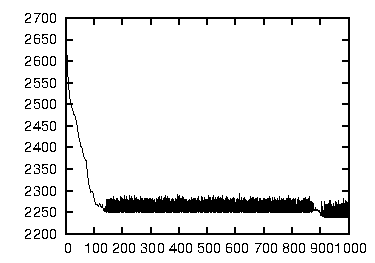
\includegraphics[scale=1.5]{plots/plot1.pdf}
  \caption{Zbieżność populacji. Zestaw t030}
  \label{pic:plot1}
\end{figure}

Podobne wnioski wyciągnęliśmy dla wszystkich posiadanych zestawów testowych. Po serii małych eksperymentów wykonaliśmy testy na znacznie większej liczbie iteracji.
Celem tych testów było sprawdzenie wydajności algorytmu SGA. Tabela \ref{tab:extreme} przedstawia wyniki przeprowadzonych eksperymentów.

\begin{figure}
  \centering
    \begin{tabular}{l|l|l|l|l|l|} \cline{2-6}
     & \multicolumn{5}{|c|}{Liczba iteracji} \\ \cline{2-6}
                                & $10^4$  & $5\cdot 10^4$ & $10^5$ & $5\cdot 10^5$ & $10^6$ \\ \hline
    \multicolumn{1}{|c|}{t001} 	& $1.48$  & $1.25$        & $1.25$ & $0.31$        & $0.00$ \\ \hline
    \multicolumn{1}{|c|}{t005} 	& $1.21$  & $1.21$        & $1.21$ & $1.05$        & -      \\ \hline
    \multicolumn{1}{|c|}{t011} 	& -  & -  & - & - & - \\ \hline
    \multicolumn{1}{|c|}{t015} 	& -  & -  & - & - & - \\ \hline
    \end{tabular}
  \caption{Odchylenie od optimum (w procentach)}
  \label{tab:extreme}
\end{figure}

\subsection{Wariancja}

Zastosowaną metryką w przestrzeni permutacji jest minimalna liczba
transpozycji potrzebnych do przekształcenia jednej permutacji w drugą.

\begin{figure}[t]
  \centering
  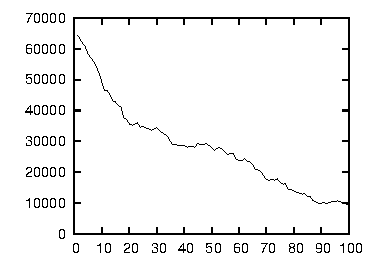
\includegraphics[scale=1.5]{plots/plot2.pdf}
  \caption{Wariancja populacji. Zestaw t013}
  \label{pic:plot2}
\end{figure}

\begin{figure}[h!]
  \centering
  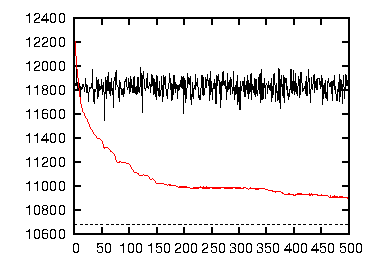
\includegraphics[scale=1.5]{plots/plot3.pdf}
  \caption{Random versus SGA. Zestaw t100}
  \label{pic:plot3}
\end{figure}

Przedstawiono wykresy wariancji populacji w tej metryce. 
Dla przykładu zamieszczmy wykres \ref{pic:plot2}, który 
przedstawia wariancję populacji dla 100 iteracji. Testy
pokazują zbieżność populacji w kolejnych iteracjach, nierzadko do
momentu, gdy cała populacja jest kopiami tego samego osobnika.

\subsection{Porównanie z losowym przeszukiwaniem przestrzeni}

Przeprowadzono testy porównujące algorytm genetyczny z losowym
przeszukiwaniem przestrzeni permutacji. Algorytm przeszukujący losowo
przestrzeń wykonywał taką samą liczbę ewaluacji jak algorytm
genetyczny. Wykres \ref{pic:plot3} pokazuje różnicę między losowym błądzeniem po przestrzeni
a algorytmem SGA dla zestawu {\em t100}. Czerwona linia jest średnią wartością funkcji celu uzyskaną
w danej iteracji przez algorytm SGA, czarna linia jest największą wartością funkcji celu uzyskaną
poprzez wykonanie tylu ewaluacji, ile osobników liczy sobie populacja w algorytmie SGA.
Otrzymano znacząco lepsze wyniki na korzyść algorytmu genetycznego.

\begin{figure}[t]
  \centering
  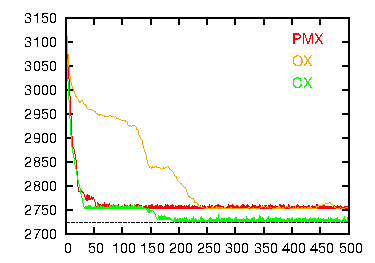
\includegraphics[scale=1.1]{plots/plot4.pdf}
  \caption{Porównanie operatorów krzyżowania, dążenie do optimum. Zestaw t031}
  \label{pic:plot4}
\end{figure}

\begin{figure}[t]
  \centering
  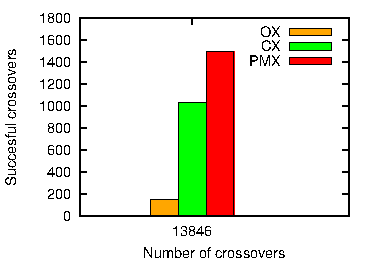
\includegraphics[scale=1.1]{plots/plot5.pdf}
  \caption{Porównanie operatorów krzyżowania, liczba udanych krzyżowań. Zestaw t097}
  \label{pic:plot5}
\end{figure}

\subsection{Jakość algorytmów krzyżowania}

Przeprowadzono testy sprawdzające, jak często wykorzystane algorytmy
krzyżowania jako wynik otrzymują osobniki lepsze od rodziców. Zostały
zaobserwowane różnice w działaniu operatorów zależnych od wyboru
wymienianego łańcucha (PMX, CX) w stosunku do operatora niezależnego
od tego wyboru (OX) (patrz wykresy \ref{pic:plot4} i \ref{pic:plot5}).
Różnica zależy od wyboru długości wymienianego łańcucha.

\end{document}
